% Provenance (never printed): old terminale S material on the transformation of
% rocks in mountain belts and subduction zones (pressure, temperature, index
% minerals and the Al2SiO5 polymorphs, foliation, contact and regional
% metamorphism). Owner (Sync 0): metamorphism, lithostatic pressure, polymorph,
% index mineral/isograd/metamorphic grade, foliation/schistosity, contact and
% regional metamorphism/aureole. Blueschist and eclogite are g11.06's, the
% geotherm g11.03's, minerals and silicates g11.07's, the rock families, marble
% and slate Book 1's (g6), pressure physics': recalled, never redefined. The
% P-T diagram: figdata/grade-12/al2sio5.py (Holdaway and Mukhopadhyay 1993,
% Table 11; geotherms from Earle 7.3).
\chapter{Batuan Metamorf}\label{ch:g12:metamorphic-rocks}

Selapis lumpur mengendap di dasar laut dan mengeras menjadi serpih. Kuburlah
lapisan itu beberapa kilometer dan jepitlah, maka lapisan itu menjadi batu
sabak, batuan yang terbelah menjadi lembaran-lembaran tipis dan datar seperti
genteng. Kuburlah lebih dalam dan lebih panas, maka serpihan-serpihannya yang
halus tumbuh menjadi mika yang berkilauan, dan di antaranya membengkak
garnet-garnet merah: sebuah sekis. Lebih dalam dan lebih panas lagi,
mineral-mineralnya memilah diri menjadi pita-pita terang dan gelap: sebuah
gneis. Tidak ada yang meleleh di sepanjang jalan itu. Lumpur yang sama, dengan
unsur-unsur kimia yang sama, hanya menyusun ulang mineral-mineralnya agar sesuai
dengan tempat ia berada. Bila dibaca ke arah sebaliknya, mineral-mineral batuan
metamorf merekam seberapa dalam dan seberapa panas tempat itu, dan bab ini
belajar membacanya.
% ledger: earle:foliation, earle:settings

\begin{recall}
Batuan terbagi menjadi tiga golongan --- beku, sedimen, metamorf --- dan
daur batuan mengubah yang satu menjadi yang lain; marmer terbentuk dari batu
kapur dan batu sabak dari serpih, tanpa meleleh (Buku 1, kelas 6). Mineral
adalah zat padat alami dengan komposisi kimia yang tetap dan susunan atom yang
teratur; sebagian besar mineral kerak adalah \omterm{def:g11:minerals:silicate}{silikat}
(\cref{ch:g11:minerals}). \omterm{def:g11:lithosphere-asthenosphere:geotherm}{Geoterm} adalah kurva suhu terhadap kedalaman di bawah
suatu tempat; di dekat permukaan suhu naik 25 sampai \qty{30}{\celsius} per
kilometer (\cref{ch:g11:lithosphere-asthenosphere}). Di \omterm{def:g11:subduction-zones:subduction}{zona subduksi}, \omterm{def:g11:ocean-ridges:oceanic-lithosphere}{kerak
samudra} yang terbawa turun selagi tetap dingin berubah menjadi \omterm{def:g11:subduction-zones:eclogite}{sekis biru}, lalu
menjadi \omterm{def:g11:subduction-zones:eclogite}{eklogit} (\cref{ch:g11:subduction-zones}). Tekanan adalah gaya dibagi
luas bidang yang ditekannya; tekanan diukur dalam pascal, \qty{1}{Pa} =
\qty{1}{N/m^2}.
\end{recall}
% ledger: usgs:metamorphic (Book 1 row), webmineral:formulas, earle:settings, earle:controls

\section{Berubah dalam keadaan padat}

\begin{definition}[Metamorfisme]\label{def:g12:metamorphic-rocks:metamorphism}
Yang disebut \emph{metamorfisme}\index{metamorfisme} adalah perubahan
mineral-mineral dan \omterm{def:g11:igneous-rocks:texture}{tekstur} sebuah batuan, dalam keadaan padat, ketika batuan
itu dibawa ke suhu dan tekanan yang berbeda dengan suhu dan tekanan tempat
batuan itu terbentuk. Batuan yang dihasilkannya adalah batuan metamorf.
\end{definition}
% ledger: tulane:metamorphism, earle:controls

Batuan yang menjadi titik awal \omterm{def:g12:metamorphic-rocks:metamorphism}{metamorfisme} adalah \omterm{def:g10:soil-formation:weathering-profile}{batuan induknya}, istilah
yang sama dengan istilah untuk batuan di bawah tanah (\cref{ch:g10:soil-formation}).
\omterm{def:g12:metamorphic-rocks:metamorphism}{Metamorfisme} dimulai pada sekitar \qty{200}{\celsius}; di bawah suhu itu,
perubahan lambat pada sedimen yang terkubur termasuk dalam proses pengerasannya
menjadi batuan. \omterm{def:g12:metamorphic-rocks:metamorphism}{Metamorfisme} berakhir di tempat batuan mulai meleleh: sejak saat
itu, yang terjadi adalah proses beku. Di antara batas-batas ini, setiap mineral
hanya stabil dalam selang suhu dan tekanan tertentu. Sebagian besar \omterm{def:g10:soil-formation:clay}{mineral
lempung}, misalnya, hanya bertahan sampai sekitar 150 atau \qty{200}{\celsius};
di atas suhu itu, mineral-mineral itu berubah menjadi mika. Ketika keadaannya
berubah, atom-atom mineral yang tidak stabil menyusun ulang dirinya, butir demi
butir, menjadi mineral-mineral yang stabil dalam keadaan yang baru.
% ledger: tulane:metamorphism, earle:controls

Empat hal mengendalikan hasilnya. \textbf{\omterm{def:g10:soil-formation:weathering-profile}{Batuan induk}} menyediakan unsur-unsur
kimia: batu kapur yang hanya tersusun dari kalsit hanya dapat menjadi marmer
yang tersusun dari kalsit. \textbf{Suhu} dan \textbf{tekanan} menentukan mineral
mana yang stabil. Dan \textbf{air}, yang ada dalam jumlah kecil di antara
butir-butir, membawa ion-ion terlarut dari satu butir ke butir berikutnya dan
mempercepat reaksi. \omterm{def:g12:metamorphic-rocks:metamorphism}{Metamorfisme} berlangsung lambat: mineral-mineral baru tumbuh
sekitar satu milimeter dalam sejuta tahun. Peristiwa tektonik yang mengubur
batuan juga lambat, sehingga reaksi-reaksi itu biasanya sempat berlangsung.
% ledger: earle:controls

\subsection{Berat batuan di atasnya}

Batuan yang terkubur pada kedalaman $z$ memikul berat semua batuan di atasnya.

\begin{definition}[Tekanan litostatik]\label{def:g12:metamorphic-rocks:lithostatic}
Yang disebut \emph{tekanan litostatik}\index{tekanan litostatik} pada kedalaman
$z$ adalah tekanan yang dikerjakan pada sebuah batuan oleh berat kolom batuan
di atasnya. Tekanan itu sama ke segala arah.
\end{definition}
% ledger: earle:controls (confining pressure, equal in all directions), tulane:metamorphism

\begin{proposition}[Tekanan litostatik]\label{prop:g12:metamorphic-rocks:lithostatic}
Di bawah kolom batuan yang massa jenisnya seragam $\rho$, \omterm{def:g12:metamorphic-rocks:lithostatic}{tekanan litostatik}
pada kedalaman $z$ adalah
\[
  P = \rho g z ,
\]
dengan $g$ percepatan gravitasi; tekanan atmosfer, sekitar \qty{0.1}{MPa},
diabaikan.
\end{proposition}

\begin{proof}
Ambillah kolom batuan tegak yang luas penampang mendatarnya $A$, dari
permukaan sampai kedalaman $z$. Volumenya $Az$, massanya $\rho A z$, dan
beratnya $\rho A z g$. Berat ini bertumpu pada luas $A$ di dasar kolom,
sehingga tekanan di sana adalah $P = \rho A z g / A = \rho g z$.
\end{proof}

Dengan massa jenis rata-rata \omterm{def:g12:continental-crust:continental-crust}{kerak benua}, $\rho = \qty{2830}{kg/m^3}$,
dan $g = \qty{9.81}{m/s^2}$, tekanan naik sebesar $\rho g = 2830 \times 9.81
\approx \qty{27800}{Pa}$ per meter, yaitu sekitar \qty{27.8}{MPa} per
kilometer. Di dasar kerak setebal \qty{35}{km} tekanan itu mencapai
\[
  P = 2830 \times 9.81 \times \num{35000} \approx \qty{9.7e8}{Pa} \approx
  \qty{0.97}{GPa},
\]
sekitar \qty{1}{GPa}: hampir sepuluh ribu kali tekanan atmosfer di permukaan
laut. Tekanan sering dibaca ke arah sebaliknya, sebagai kedalaman:
\qty{1}{GPa} tercapai pada kedalaman $\num{e9}/(2830 \times 9.81) \approx \qty{36}{km}$.
% values: P_35km_gpa 0.97168, dPdz_mpa_per_km 27.762, z_1gpa_km 36.02 (al2sio5.py)
% ledger: cm95:crust; Book 1: ussa76:sea-level (101 325 Pa, g0 = 9.80665 m/s2)

Berat batuan menekan sama kuat dari segala sisi. Di sabuk pegunungan,
lempeng-lempeng menambahkan dorongan ke satu arah: batuan terjepit lebih kuat
dari samping daripada dari atas. Tekanan \emph{berarah} ini tidak mengubah
mineral mana yang stabil, tetapi mengubah cara mineral-mineral itu tersusun,
seperti yang ditunjukkan \cref{sec:g12:metamorphic-rocks:foliation}.
% ledger: earle:controls (directed pressure), earle:foliation

\section{Mineral indeks dan derajat metamorfisme}

\subsection{Tiga mineral dengan satu rumus}

\begin{definition}[Polimorf]\label{def:g12:metamorphic-rocks:polymorph}
Dua mineral disebut \emph{polimorf}\index{polimorf} bila keduanya mempunyai
komposisi kimia yang sama tetapi struktur kristal yang berbeda: atom-atom yang
sama, yang tersusun secara berbeda.
\end{definition}
% ledger: earle:controls

Tiga mineral mempunyai rumus yang sama, \ce{Al2SiO5}: kianit, andalusit, dan
silimanit. Masing-masing stabil dalam selang suhu dan tekanannya sendiri, yang
diukur di laboratorium dengan menahan kristal-kristal pada suhu dan tekanan
yang dipilih dan mengamati \omterm{def:g12:metamorphic-rocks:polymorph}{polimorf} mana yang tumbuh dengan mengorbankan yang
lain. Kianit adalah yang paling rapat di antara ketiganya,
\qty{3.61}{g/cm^3} dibandingkan dengan \qty{3.24}{g/cm^3} untuk silimanit dan
\qty{3.15}{g/cm^3} untuk andalusit: atom-atomnya tersusun lebih rapat, dan
kianitlah yang diuntungkan oleh tekanan tinggi.
% ledger: earle:controls, hm93:triple, hm93:table11; Book 3: webmineral:polymorphs (densities)

\begin{omfigure}
\begin{tikzpicture}
\begin{axis}[omrecord, name=pt, scale only axis, width=0.62\linewidth, height=6.4cm,
  xmin=200, xmax=900, ymin=0, ymax=1.2, y dir=reverse,
  xlabel={suhu (\unit{\celsius})}, ylabel={tekanan (\unit{GPa})},
  xtick={200,300,...,900}, ytick={0,0.2,...,1.2},
  yticklabel style={/pgf/number format/fixed, /pgf/number format/precision=1},
  axis y line*=left]
% computed in figdata/grade-12/al2sio5.py from Holdaway and Mukhopadhyay (1993), Table 11
\addplot[omDef, line width=0.9pt, densely dashed] table[x=T10, y=P_GPa] {figdata/out/grade-12-al2sio5-geotherms.dat};
\addplot[omMeth, line width=0.9pt, densely dashed] table[x=T30, y=P_GPa] {figdata/out/grade-12-al2sio5-geotherms.dat};
\addplot[omThm, line width=0.9pt, densely dashed] table[x=T50, y=P_GPa] {figdata/out/grade-12-al2sio5-geotherms.dat};
\addplot[black, line width=1.2pt] table[x=T, y=P_GPa] {figdata/out/grade-12-al2sio5-andky.dat};
\addplot[black, line width=1.2pt] table[x=T, y=P_GPa] {figdata/out/grade-12-al2sio5-kysil.dat};
\addplot[black, line width=1.2pt] table[x=T, y=P_GPa] {figdata/out/grade-12-al2sio5-andsil.dat};
\addplot[black, line width=1.2pt, dotted] table[x=T, y=P_GPa] {figdata/out/grade-12-al2sio5-andsilx.dat};
\addplot[only marks, mark=*, mark size=2pt, black] coordinates {(504.2,0.3758)};
\addplot[only marks, mark=o, mark size=2pt, line width=0.8pt, black] coordinates {(573.6,0.5216) (340.1,0.1833) (553.0,0.3015)};
\coordinate (ky) at (axis cs:370,0.55);
\coordinate (and) at (axis cs:470,0.12);
\coordinate (sil) at (axis cs:765,0.57);
\coordinate (tp) at (axis cs:504.2,0.3758);
\coordinate (g10) at (axis cs:415,1.0);
\coordinate (g30) at (axis cs:206,0.36);
\coordinate (g50) at (axis cs:895,0.355);
\end{axis}
\begin{axis}[scale only axis, width=0.62\linewidth, height=6.4cm, at={(pt.south west)}, anchor=south west,
  xmin=200, xmax=900, ymin=0, ymax=43.224, y dir=reverse, axis x line=none, axis y line*=right,
  axis line style={-}, ylabel={kedalaman (\unit{km})}, ytick={0,5,...,40},
  every axis label/.append style={font=\small}, tick label style={font=\small}]
\end{axis}
\node[font=\small\bfseries] at (ky) {kianit};
\node[font=\small\bfseries] at (and) {andalusit};
\node[font=\small\bfseries] at (sil) {silimanit};
\node[font=\scriptsize, text=omDef, anchor=west, inner sep=1pt] at (g10) {\qty{10}{\celsius/km}, zona subduksi};
\node[font=\scriptsize, text=omMeth!70!black, anchor=north west, inner sep=1pt, align=left] at (g30) {\qty{30}{\celsius/km},\\umum};
\node[font=\scriptsize, text=omThm, anchor=south east, inner sep=1pt] at (g50) {\qty{50}{\celsius/km}, daerah gunung api};
\end{tikzpicture}

{\small Medan-medan ketiga \omterm{def:g12:metamorphic-rocks:polymorph}{polimorf} \ce{Al2SiO5}, dengan tekanan yang bertambah
ke bawah seperti kedalaman (skala di sebelah kanan, untuk kerak bermassa jenis
\qty{2830}{kg/m^3}). Garis hitam: batas-batas yang diukur di laboratorium;
ketiganya bertemu di titik tripel (titik hitam), \qty{504}{\celsius} dan
\qty{0.375}{GPa}. Garis putus-putus: tiga \omterm{def:g11:lithosphere-asthenosphere:geotherm}{geoterm}, yang bermula dari
\qty{10}{\celsius} di permukaan; lingkaran-lingkaran menandai tempat \omterm{def:g11:lithosphere-asthenosphere:geotherm}{geoterm}
itu memotong sebuah batas.}
\end{omfigure}
% values: triple_T 504.21, triple_P_gpa 0.37584, triple_z_km 13.538; crossings 30: 573.6 degC 18.79 km; 50: 340.1 degC 6.60 km, 553.0 degC 10.86 km (al2sio5.py)
% ledger: hm93:table11, hm93:triple, cm95:crust, earle:settings

Diagram itu adalah peta kestabilan. Setiap titik adalah sebuah suhu dan sebuah
tekanan; setiap medan adalah \omterm{def:g12:metamorphic-rocks:polymorph}{polimorf} yang stabil di sana. Kianit menempati
tekanan tinggi, andalusit tekanan rendah dan suhu sedang, silimanit suhu
tinggi. Di sepanjang sebuah batas, dua \omterm{def:g12:metamorphic-rocks:polymorph}{polimorf} sama stabilnya, dan di titik
tripel, ketiganya. Batas-batas itu tidak diketahui secara persis: titik tripel
itu tidak pasti sekitar \qty{20}{\celsius} dan \qty{0.025}{GPa}, dan jejak besi
dalam kristal menggeser garis andalusit--silimanit sampai \qty{20}{\celsius}.
% ledger: hm93:triple

\begin{method}[Membaca diagram tekanan--suhu]\label{met:g12:metamorphic-rocks:pt}
\begin{enumerate}
  \item Tempatkan titik batuan itu: suhunya pada sumbu mendatar, tekanannya
        pada sumbu tegak.
  \item Bacalah medan tempat titik itu jatuh: mineral yang stabil di sana.
  \item Ubahlah tekanan menjadi kedalaman dengan $z = P/(\rho g)$, atau
        bacalah pada skala kedalaman.
  \item Untuk mineral yang ditemukan dalam batuan, bacalah ke arah sebaliknya:
        batuan itu berada di medan mineral tersebut ketika mineral itu
        mengkristal. Dua mineral yang terbentuk bersama, atau mineral yang
        tidak ada, mempersempit selangnya lebih jauh.
\end{enumerate}
\end{method}

\begin{example}[Batas kianit--silimanit]\label{ex:g12:metamorphic-rocks:kysil}
Pada \qty{0.6}{GPa}, kianit berubah menjadi silimanit pada sekitar
\qty{611}{\celsius}. Tekanan itu tercapai pada $z = \num{0.6e9} / (2830
\times 9.81) \approx \qty{21.6}{km}$. Antara 600 dan \qty{700}{\celsius}
batas itu naik sebesar \qty{0.209}{GPa}, yaitu $0.209/0.0278 \approx
\qty{7.5}{km}$ kedalaman: batuan yang \qty{7.5}{km} lebih dalam harus sekitar
\qty{100}{\celsius} lebih panas untuk berubah menjadi silimanit. Sekis yang
mengandung kianit tetapi tidak mengandung silimanit dan mengkristal pada
\qty{21.6}{km} karena itu lebih dingin daripada sekitar \qty{611}{\celsius}.
\end{example}
% values: kysil_T_at_6kbar 611, kysil_z_at_6kbar 21.612, kysil_slope 2.09 kbar per 100 degC, dPdz 27.762 MPa/km (al2sio5.py)

\subsection{Mineral indeks dan isograd}

Di sebuah sabuk batuan yang semuanya berasal dari lumpur yang sama,
mineral-mineralnya berubah dari tempat ke tempat, karena batuan-batuan itu
tidak terkubur sama dalam atau terpanaskan sama kuat.

\begin{definition}[Mineral indeks; isograd; derajat metamorfisme]\label{def:g12:metamorphic-rocks:index-mineral}
Yang disebut \emph{derajat metamorfisme}\index{derajat metamorfisme} sebuah
batuan adalah intensitas \omterm{def:g12:metamorphic-rocks:metamorphism}{metamorfisme} yang dialaminya, yang ditentukan oleh
suhu dan tekanan yang dicapainya. Yang disebut \emph{mineral
indeks}\index{mineral indeks} adalah mineral yang kemunculan pertamanya, pada
batuan dengan komposisi induk yang sama, menandai suatu derajat tertentu. Yang
disebut \emph{isograd}\index{isograd} adalah garis pada peta (sebuah bidang di
dalam tanah) yang menghubungkan tempat-tempat mineral indeks pertama kali
muncul: di sepanjang garis itu, batuan-batuan telah mencapai derajat yang sama.
\end{definition}
% ledger: tulane:metamorphism, earle:regional

Batuan yang terbentuk dari lumpur, yang kaya aluminium, memperlihatkan urutan
yang paling jelas. Dengan derajat yang naik, mineral-mineral indeks muncul
dalam urutan klorit, biotit, garnet, staurolit, kianit, silimanit, dan daerah
yang dibaginya disebut zona klorit, zona biotit, dan seterusnya. Suhu dan
tekanan sama-sama naik di sepanjang urutan itu, seperti yang terjadi pada kerak
yang menebal di bawah sabuk pegunungan.
% ledger: iugs:barrow, earle:regional

\begin{omfigure}
\begin{tikzpicture}[font=\scriptsize]
  \def\zone#1#2#3#4{\fill[#1] (#2,0) ellipse ({#3} and {#4});}
  \zone{omProp!8}{0}{6.6}{2.55}
  \zone{omProp!18}{0.5}{5.4}{2.2}
  \zone{omProp!32}{1.0}{4.3}{1.82}
  \zone{omThm!28}{1.4}{3.2}{1.44}
  \zone{omThm!45}{1.8}{2.1}{1.06}
  \zone{omThm!65}{2.2}{1.0}{0.66}
  \foreach \c/\a/\b in {0.5/5.4/2.2, 1.0/4.3/1.82, 1.4/3.2/1.44, 1.8/2.1/1.06, 2.2/1.0/0.66}
    \draw[black!70, line width=0.6pt] (\c,0) ellipse ({\a} and {\b});
  \draw[black!40] (0,0) ellipse (6.6 and 2.55);
  \node at (-5.75,0) {klorit};
  \node at (-4.1,0) {biotit};
  \node at (-2.55,0) {garnet};
  \node at (-1.05,0) {staurolit};
  \node at (0.45,0) {kianit};
  \node[text=white, font=\scriptsize\bfseries] at (2.2,0) {silimanit};
  \draw[omDef, -{Stealth}, line width=0.8pt] (5.6,-2.6) node[right, text=omDef] {derajat naik} -- (3.0,-0.65);
  \draw[black!70] (3.76,1.394) -- (5.8,2.2) node[right, align=left] {isograd\\garnet};
\end{tikzpicture}

{\small Peta skematis zona-zona \omterm{def:g12:metamorphic-rocks:metamorphism}{metamorfisme} pada batuan yang terbentuk dari
lumpur: setiap \omterm{def:g12:metamorphic-rocks:index-mineral}{isograd} (garis hitam) menandai kemunculan pertama sebuah \omterm{def:g12:metamorphic-rocks:index-mineral}{mineral
indeks}, dan derajatnya naik ke arah inti sabuk, tempat batuan-batuan terkubur
paling dalam dan terpanaskan paling kuat. Zona-zona yang sebenarnya melengkung
dan terpotong oleh \omterm{def:g12:mountain-building:fold}{lipatan} dan sesar; lebarnya di sini sembarang.}
\end{omfigure}
% ledger: iugs:barrow, earle:regional

\begin{history}[Zona-zona Barrow]
Pada tahun 1890-an, ahli geologi George Barrow memetakan sekis dan gneis di
Dataran Tinggi Skotlandia dan memperhatikan bahwa mineral-mineralnya berubah
melintasi daerah itu dalam urutan yang teratur. Dialah orang pertama yang
membagi sebuah wilayah menjadi zona-zona menurut mineral yang dikandung
batuannya. Namanya diabadikan untuk urutan itu: batuan yang mengikutinya
dikatakan memperlihatkan \omterm{def:g12:metamorphic-rocks:metamorphism}{metamorfisme} \emph{tipe Barrow}.
\end{history}
% ledger: earle:regional, barrow1893:paper, iugs:barrow

\omterm{def:g12:metamorphic-rocks:index-mineral}{Derajat metamorfisme} juga dapat diperkirakan secara kasar dari suhu saja.
Batuan yang terpanaskan sampai 150 hingga \qty{300}{\celsius} berderajat sangat
rendah, 300 hingga \qty{450}{\celsius} berderajat rendah, 450 hingga
\qty{550}{\celsius} berderajat sedang, dan di atas \qty{550}{\celsius}
berderajat tinggi. Pada derajat rendah batuan kaya akan mineral yang menyimpan
air dalam strukturnya, seperti lempung dan klorit; ketika derajatnya naik,
batuan itu kehilangan air tersebut.
% ledger: earle:foliation (Table 7.1 grades), tulane:metamorphism

\section{Foliasi}\label{sec:g12:metamorphic-rocks:foliation}

Bila terjepit selagi tumbuh, mineral-mineral tidak tumbuh ke segala arah.
Butir-butir pipih seperti mika, dan butir-butir panjang seperti amfibol,
mengkristal dengan bidang pipihnya atau sumbu panjangnya melintang terhadap
arah dorongan; butir-butir yang sudah ada sebelumnya memipih dengan cara yang
sama.
% ledger: earle:foliation, tulane:metamorphism

\begin{definition}[Foliasi; skistositas]\label{def:g12:metamorphic-rocks:foliation}
Yang disebut \emph{foliasi}\index{foliasi} adalah sekumpulan bidang sejajar
dalam batuan metamorf, yang terbentuk oleh penjajaran mineral-mineralnya yang
pipih atau memanjang; batuan itu paling mudah terbelah di sepanjang
bidang-bidang tersebut. Yang disebut \emph{skistositas}\index{skistositas}
adalah foliasi sebuah sekis, yang kristal-kristal mikanya yang berjajar cukup
besar untuk dilihat.
\end{definition}
% ledger: earle:foliation, tulane:metamorphism

\begin{omfigure}
\begin{tikzpicture}[font=\scriptsize]
  \pgfmathsetseed{4}
  % before: random flakes in a square
  \draw[black!60, fill=omLithShale!35] (0,0) rectangle (3.2,3.2);
  \foreach \i in {1,...,38} {
    \pgfmathsetmacro{\x}{0.3+2.6*rnd}\pgfmathsetmacro{\y}{0.3+2.6*rnd}\pgfmathsetmacro{\a}{180*rnd}
    \draw[black!75, line width=1.1pt] ($(\x,\y)+(\a:0.2)$) -- ($(\x,\y)+(\a+180:0.2)$);
  }
  \foreach \i in {1,...,14} {
    \pgfmathsetmacro{\x}{0.3+2.6*rnd}\pgfmathsetmacro{\y}{0.3+2.6*rnd}
    \fill[white, draw=black!40] (\x,\y) circle (0.07);
  }
  \node[below] at (1.6,-0.3) {sebelum: serpihan ke segala arah};
  % after: squeezed from the sides
  \begin{scope}[xshift=7.3cm]
  \draw[black!60, fill=omLithSchist!45] (0,-0.3) rectangle (2.4,3.5);
  \foreach \i in {1,...,38} {
    \pgfmathsetmacro{\x}{0.2+2.0*rnd}\pgfmathsetmacro{\y}{0.1+3.0*rnd}\pgfmathsetmacro{\a}{90+12*(rnd-0.5)}
    \draw[black!75, line width=1.1pt] ($(\x,\y)+(\a:0.24)$) -- ($(\x,\y)+(\a+180:0.24)$);
  }
  \foreach \i in {1,...,14} {
    \pgfmathsetmacro{\x}{0.2+2.0*rnd}\pgfmathsetmacro{\y}{0.1+3.0*rnd}
    \fill[white, draw=black!40] (\x,\y) ellipse (0.045 and 0.09);
  }
  \draw[omThm, -{Stealth}, line width=1.4pt] (-1.1,1.6) -- (-0.15,1.6);
  \draw[omThm, -{Stealth}, line width=1.4pt] (3.5,1.6) -- (2.55,1.6);
  \node[below] at (1.2,-0.3) {sesudah: serpihan melintang terhadap jepitan};
  \node[omThm, above] at (-0.65,1.65) {dorongan};
  \node[omThm, above] at (3.05,1.65) {dorongan};
  \end{scope}
  \draw[-{Stealth}, black!50, line width=0.8pt] (3.5,1.6) -- node[above] {dipanaskan dan} node[below] {dijepit} (5.2,1.6);
\end{tikzpicture}

{\small Terbentuknya \omterm{def:g12:metamorphic-rocks:foliation}{foliasi}. Kiri: lumpur dengan serpihan lempung (hitam) dan
butir kuarsa (putih) yang terletak ke segala arah. Kanan: dijepit dari samping
selagi dipanaskan, batuan itu menumbuhkan serpihan mika yang melintang terhadap
dorongan dan memipihkan butir-butirnya: kini batuan itu terbelah di sepanjang
bidang-bidang tegak.}
\end{omfigure}
% ledger: earle:foliation

Lumpur, yang kaya serpihan lempung yang pipih, memperlihatkan urutan itu paling
baik. Dengan derajat yang naik, lumpur itu berturut-turut menjadi:
\begin{itemize}
  \item \textbf{batu sabak}, yang serpihan lempung dan mikanya yang berjajar
        terlalu kecil untuk dilihat; batu sabak terbelah menjadi lembaran datar;
  \item \textbf{filit}, yang mikanya telah tumbuh cukup besar untuk memberi
        \omterm{def:g11:minerals:lustre}{kilap} seperti sutra;
  \item \textbf{sekis}, yang mikanya terlihat, sering kali dengan kristal garnet,
        kianit, atau staurolit yang lebih besar di antaranya;
  \item \textbf{gneis}, yang mineral-mineralnya telah terpisah menjadi pita
        terang (kuarsa, feldspar) dan pita gelap, dan yang mengandung sedikit
        mika atau tidak sama sekali, karena terlalu panas bagi mika untuk
        bertahan.
\end{itemize}
% ledger: earle:foliation, earle:settings (slate 5-10 km to gneiss 20-25 km on a typical gradient)

\begin{omfigure}
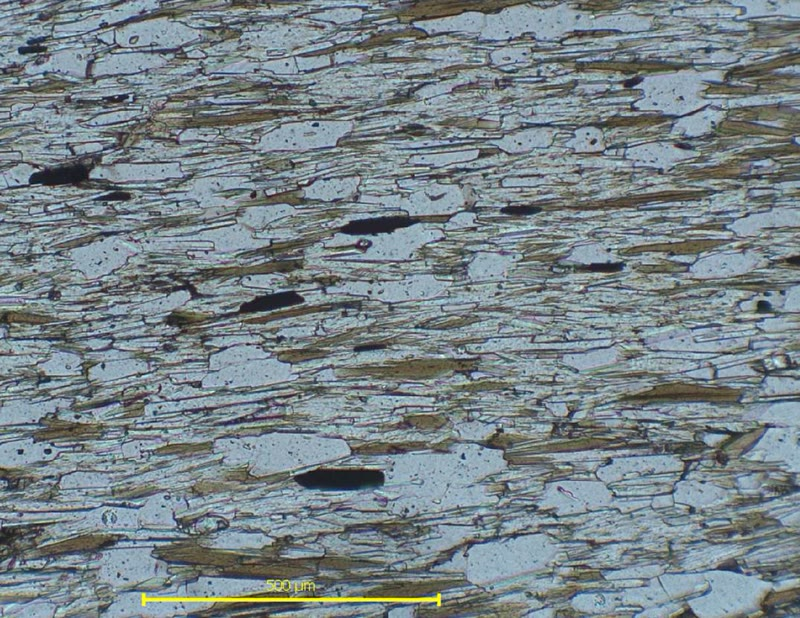
\includegraphics[height=4.3cm]{images/book2/g12-geoloshe-slaty-cleavage.jpg}\hspace{0.03\linewidth}%
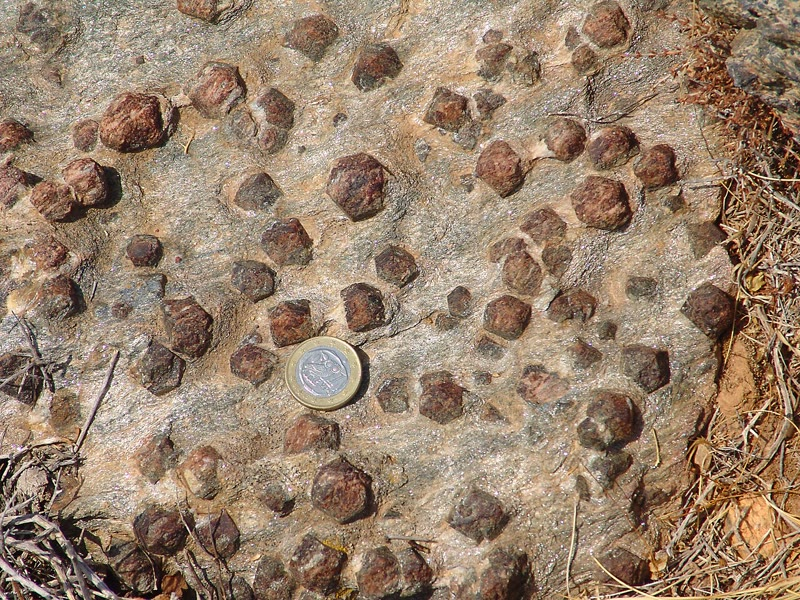
\includegraphics[height=4.3cm]{images/book2/g12-churchard-syros-garnet-schist.jpg}

\smallskip
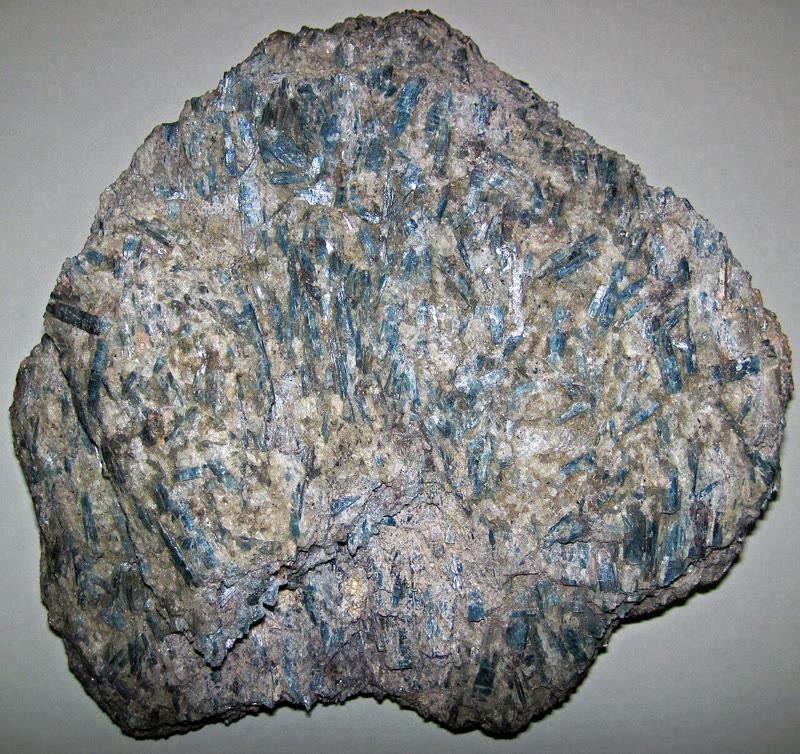
\includegraphics[height=4.3cm]{images/book2/g12-stjohn-kyanite-schist.jpg}\hspace{0.03\linewidth}%
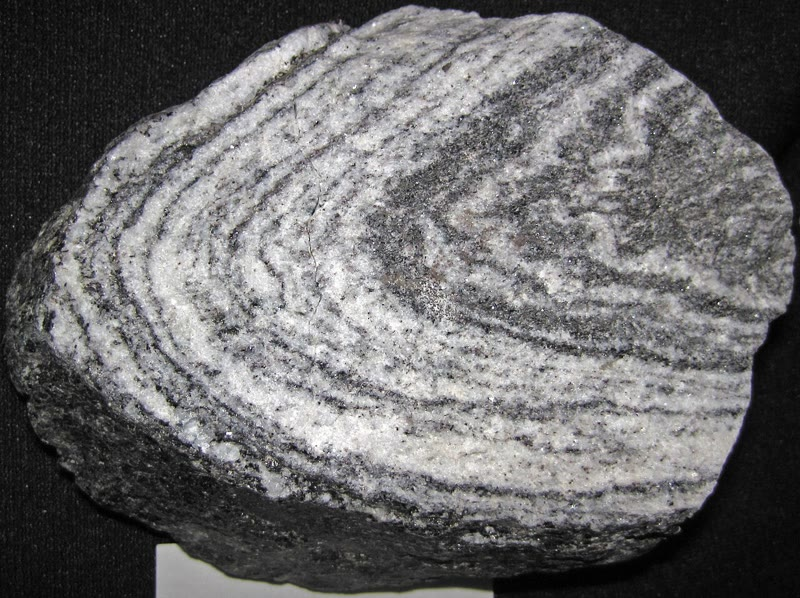
\includegraphics[height=4.3cm]{images/book2/g12-stjohn-gneiss.jpg}

{\small Kiri atas: batu sabak di bawah mikroskop (batang kuning panjangnya
\qty{500}{\micro\metre}): serpihan-serpihan mikanya semuanya terletak searah.
Kanan atas: sekis mika bergarnet di Pulau Syros; lebar koin itu
\qty{23}{mm}. Kiri bawah: sekis dengan bilah-bilah kianit berwarna biru.
Kanan bawah: gneis dengan pita-pita kuarsa (terang) dan mika biotit (gelap).
Foto Geoloshe (CC0), Graeme Churchard (CC~BY~2.0), dan James St.~John
(CC~BY~2.0).}
\end{omfigure}
% ledger: photo:g12-slaty-cleavage, photo:g12-syros-schist, photo:g12-kyanite-schist, photo:g12-gneiss

Di sepanjang \omterm{def:g11:lithosphere-asthenosphere:geotherm}{geoterm} yang umum, batu sabak terbentuk antara sekitar 5 dan
\qty{10}{km} di bawah permukaan, filit antara 10 dan 15, sekis antara 15 dan
20, dan gneis antara 20 dan \qty{25}{km}; lebih dalam lagi, batuan mulai
meleleh di beberapa tempat. \omterm{def:g12:metamorphic-rocks:foliation}{Foliasi} merekam arah jepitan: \omterm{def:g12:metamorphic-rocks:foliation}{foliasi} terbentuk
melintang terhadap \omterm{def:g12:mountain-building:shortening}{pemendekan} yang membangun pegunungan
(\cref{ch:g12:mountain-building}), dan perlapisan asli lumpur itu mungkin masih
terlihat memotongnya dengan sudut tertentu.
% ledger: earle:settings, earle:foliation

Batuan tanpa mineral pipih atau panjang tidak memperlihatkan \omterm{def:g12:metamorphic-rocks:foliation}{foliasi} walaupun
terjepit. Batu kapur menjadi \textbf{marmer}, yang tersusun dari kristal-kristal
kalsit yang lebih besar dan fosil-fosilnya telah terhapus; batu pasir menjadi
\textbf{kuarsit}, yang butir-butir kuarsanya telah tumbuh saling menyatu; dan
lumpur yang dipanaskan tanpa dijepit menjadi batuan keras berbutir halus tanpa
\omterm{def:g12:metamorphic-rocks:foliation}{foliasi}, yaitu \textbf{hornfels}.
% ledger: earle:foliation, earle:contact

\section{Metamorfisme kontak dan metamorfisme regional}

\begin{definition}[Metamorfisme kontak; metamorfisme regional; aureol]\label{def:g12:metamorphic-rocks:contact-regional}
Yang disebut \emph{metamorfisme kontak}\index{metamorfisme kontak} adalah
\omterm{def:g12:metamorphic-rocks:metamorphism}{metamorfisme} batuan yang terpanaskan oleh tubuh magma yang menerobosnya;
\omterm{def:g12:metamorphic-rocks:metamorphism}{metamorfisme} ini terbatas pada sebuah zona di sekitar \omterm{def:g11:igneous-rocks:intrusion}{intrusi}, yaitu
\emph{aureol}\index{aureol}-nya, yang derajatnya naik ke arah bidang kontak.
Yang disebut \emph{metamorfisme regional}\index{metamorfisme regional}
memengaruhi batuan yang terkubur dalam di wilayah yang luas, biasanya di tempat
lempeng-lempeng saling mendekat; batuannya terjepit sekaligus terpanaskan, dan
hampir selalu berfoliasi.
\end{definition}
% ledger: earle:contact, earle:regional, tulane:metamorphism

\subsection{Di sekitar tubuh magma}

Tubuh magma bersuhu sekitar \qty{1000}{\celsius} yang naik ke dalam kerak atas
yang dingin memanaskan batuan di sekitarnya. Suhunya dapat mencapai 300 sampai
lebih dari \qty{800}{\celsius}, pada tekanan rendah kedalaman yang dangkal.
\omterm{def:g12:metamorphic-rocks:contact-regional}{Aureolnya} sempit: beberapa sentimeter di sekitar lembaran magma yang tipis,
sampai beberapa puluh meter di sekitar tubuh yang besar. Batuannya terpanaskan
tanpa terjepit, sehingga tidak berfoliasi: lumpur menjadi hornfels, batu kapur
menjadi marmer, batu pasir menjadi kuarsit. Tubuh magma yang menetap jauh di
dalam batuan yang sudah panas hampir tidak membentuk \omterm{def:g12:metamorphic-rocks:contact-regional}{aureol}.
% ledger: earle:contact, earle:settings (magma bodies around 1000 degC)

\begin{omfigure}
\begin{tikzpicture}[font=\scriptsize]
  \def\pluton{(3.0,0) .. controls (3.0,2.3) and (7.0,2.3) .. (7.0,0) -- cycle}
  \def\aureole{(2.45,0) .. controls (2.45,2.95) and (7.55,2.95) .. (7.55,0) -- cycle}
  \fill[lith sandstone] (0,0) rectangle (10,0.8);
  \fill[lith limestone] (0,0.8) rectangle (10,1.6);
  \fill[lith shale] (0,1.6) rectangle (10,3);
  \fill[omThm, opacity=0.30] \aureole;
  \draw[omThm, line width=0.6pt, dashed] (2.45,0) .. controls (2.45,2.95) and (7.55,2.95) .. (7.55,0);
  \fill[lith granite] \pluton;
  \draw[black!70, line width=0.6pt] (3.0,0) .. controls (3.0,2.3) and (7.0,2.3) .. (7.0,0);
  \draw[black!60] (0,0) rectangle (10,3);
  \node[fill=white, inner sep=1.5pt] at (5,0.45) {granit (dahulu magma)};
  \draw[black!70] (6.0,1.95) -- (10.6,2.4) node[right] {hornfels, dari lumpur};
  \draw[black!70] (7.0,1.2) -- (10.6,1.2) node[right] {marmer, dari batu kapur};
  \draw[black!70] (7.25,0.4) -- (10.6,0.4) node[right] {kuarsit, dari batu pasir};
  \node[left] at (0,2.3) {serpih};
  \node[left] at (0,1.2) {batu kapur};
  \node[left] at (0,0.4) {batu pasir};
  \draw[omThm] (4.2,2.05) -- (3.4,3.25) node[above, omThm] {aureol};
\end{tikzpicture}

{\small \omterm{def:g12:metamorphic-rocks:contact-regional}{Metamorfisme kontak}, dalam penampang: sebuah tubuh magma telah naik ke
dalam batuan sedimen berlapis dan memanaskan \omterm{def:g12:metamorphic-rocks:contact-regional}{aureol} yang sempit (merah) di
sekitarnya, yang batuannya mengkristal ulang tanpa terjepit. Skematis: \omterm{def:g12:metamorphic-rocks:contact-regional}{aureol}
yang sebenarnya selebar beberapa sentimeter sampai puluhan meter.}
\end{omfigure}
% ledger: earle:contact

\subsection{Di bawah sabuk pegunungan}

\omterm{def:g12:metamorphic-rocks:contact-regional}{Metamorfisme regional} memerlukan penimbunan sampai 10 atau \qty{20}{km},
sehingga memengaruhi ribuan kilometer persegi sekaligus. Tempat yang paling
mungkin adalah \omterm{def:g12:continental-crust:root}{akar} sabuk pegunungan, tempat tumbukan menebalkan kerak dan
mendorong batuannya ke bawah (\cref{ch:g12:mountain-building}). Di sebuah sabuk
tua yang zona-zonanya telah dipetakan, batuan zona silimanit terpanaskan di
atas \qty{700}{\celsius} dan terkubur sedalam 20 sampai \qty{25}{km},
sedangkan batuan zona klorit di bagian luar kemungkinan tidak pernah terkubur
lebih dari sekitar \qty{5}{km}. Pegunungan di atasnya kemudian terkikis selama
puluhan juta tahun; ketika bebannya tersingkir, kerak yang tebal itu naik lagi,
dan zona-zona yang dahulu dalam kini terletak di permukaan
(\cref{ch:g12:destruction-of-mountains}).
% ledger: earle:regional

\subsection{Tiga geoterm}

\omterm{def:g12:metamorphic-rocks:polymorph}{Polimorf-polimorf} itu langsung menunjukkan bahwa kedalaman yang sama tidak
berarti batuan yang sama di mana-mana: hal itu bergantung pada \omterm{def:g11:lithosphere-asthenosphere:geotherm}{geotermnya}.
Gambar \omterm{def:g12:metamorphic-rocks:polymorph}{polimorf} di atas memuat tiga \omterm{def:g11:lithosphere-asthenosphere:geotherm}{geoterm}.
% ledger: earle:settings

\begin{itemize}
  \item \omterm{def:g11:lithosphere-asthenosphere:geotherm}{Geoterm} yang \textbf{umum}, sekitar \qty{30}{\celsius} per
        kilometer: suhunya mencapai sekitar \qty{300}{\celsius} pada
        \qty{10}{km}. \omterm{def:g11:lithosphere-asthenosphere:geotherm}{Geoterm} ini melewati bagian bawah titik tripel, sehingga
        kianit langsung berganti menjadi silimanit, pada sekitar
        \qty{574}{\celsius} dan \qty{18.8}{km}.
  \item \omterm{def:g11:lithosphere-asthenosphere:geotherm}{Geoterm} \textbf{daerah gunung api}, 40 sampai \qty{50}{\celsius} per
        kilometer, yang dicuramkan oleh kalor magma yang naik: batuan mencapai
        suhu tinggi pada kedalaman yang dangkal. Pada \qty{50}{\celsius} per
        kilometer, andalusit muncul pada sekitar \qty{6.6}{km} dan berganti
        menjadi silimanit pada sekitar \qty{10.9}{km}, \qty{553}{\celsius}.
  \item \omterm{def:g11:lithosphere-asthenosphere:geotherm}{Geoterm} \textbf{\omterm{def:g11:subduction-zones:subduction}{zona subduksi}}, di bawah
        \qty{10}{\celsius} per kilometer: \omterm{def:g11:ocean-ridges:oceanic-lithosphere}{kerak samudra} yang terbawa turun tetap
        beberapa ratus derajat lebih dingin daripada mantel di sekitarnya. Pada
        \qty{36}{km} suhunya hanya sekitar \qty{370}{\celsius}, jauh di dalam
        medan kianit. Inilah jalur dingin bertekanan tinggi yang membuat basalt
        menjadi \omterm{def:g11:subduction-zones:eclogite}{sekis biru}, lalu \omterm{def:g11:subduction-zones:eclogite}{eklogit}, pada sekitar \qty{35}{km}.
\end{itemize}
% values: cross_30_0 573.6 degC 18.79 km; cross_50_0 340.1 degC 6.60 km; cross_50_1 553.0 degC 10.86 km; sub10_T_at_1gpa 370.2 (al2sio5.py)
% ledger: earle:settings

Jadi setiap batuan metamorf membawa catatan tentang \omterm{def:g11:lithosphere-asthenosphere:geotherm}{geoterm} tempat batuan itu
terbentuk, dan tentang tatanan lempeng di baliknya: andalusit dan hornfels
menunjuk pada kalor di kedalaman yang dangkal, di sekitar tubuh magma; sekis dan
gneis berkianit dan bersilimanit pada \omterm{def:g12:continental-crust:root}{akar-akar} dalam sabuk pegunungan; \omterm{def:g11:subduction-zones:eclogite}{sekis
biru} dan \omterm{def:g11:subduction-zones:eclogite}{eklogit} pada \omterm{def:g11:subduction-zones:subduction}{zona subduksi}. Sebagian besar batuan ini hanya dapat
dilihat karena kembali ke permukaan tanpa berubah kembali. Ketika batuan itu
naik dan mendingin, reaksinya melambat, dan air yang diperlukan reaksi
kebalikannya telah lolos dalam perjalanan turun.
% ledger: earle:settings, earle:contact, tulane:metamorphism (retrograde metamorphism uncommon)

\section{Latihan}

\begin{exercise}[$\star$]\label{exo:g12:metamorphic-rocks:1}
Sebutkan istilahnya: (a) mineral-mineral dengan komposisi yang sama tetapi
struktur kristal yang berbeda; (b) garis pada peta tempat \omterm{def:g12:metamorphic-rocks:index-mineral}{mineral indeks}
pertama kali muncul; (c) zona batuan yang terpanaskan di sekitar tubuh magma;
(d) bidang-bidang sejajar yang terbentuk oleh mineral pipih yang berjajar;
(e) tekanan akibat berat batuan di atasnya.
\end{exercise}

\begin{exercise}[$\star$]\label{exo:g12:metamorphic-rocks:2}
Sebutkan batuan metamorf yang terbentuk dari setiap \omterm{def:g10:soil-formation:weathering-profile}{batuan induk}: (1) batu
kapur; (2) batu pasir; (3) lumpur, pada derajat rendah di bawah jepitan;
(4) lumpur, pada derajat tinggi; (5) lumpur, yang terpanaskan oleh tubuh magma
tanpa terjepit.
\end{exercise}

\begin{exercise}[$\star$]\label{exo:g12:metamorphic-rocks:3}
Dengan $\rho = \qty{2830}{kg/m^3}$ dan $g = \qty{9.81}{m/s^2}$, hitung \omterm{def:g12:metamorphic-rocks:lithostatic}{tekanan
litostatik}, dalam \unit{GPa}, pada \qty{10}{km} dan pada \qty{20}{km}.
\end{exercise}

\begin{exercise}[$\star$]\label{exo:g12:metamorphic-rocks:4}
Pada diagram \omterm{def:g12:metamorphic-rocks:polymorph}{polimorf} \ce{Al2SiO5}, mineral manakah yang stabil
(1) pada \qty{400}{\celsius} dan \qty{0.6}{GPa}; (2) pada \qty{500}{\celsius}
dan \qty{0.2}{GPa}; (3) pada \qty{750}{\celsius} dan \qty{0.3}{GPa}?
\end{exercise}

\begin{exercise}[$\star$]\label{exo:g12:metamorphic-rocks:5}
(1) Urutkan menurut derajat yang naik: sekis, batu sabak, gneis, filit.
(2) Pada batuan mana mikanya dapat dilihat dengan mata telanjang? (3) Batuan
mana yang memperlihatkan pita terang dan gelap?
\end{exercise}

\begin{exercise}[$\star\star$]\label{exo:g12:metamorphic-rocks:6}
(1) Hitung \omterm{def:g12:metamorphic-rocks:lithostatic}{tekanan litostatik} di dasar kerak setebal \qty{35}{km}
($\rho = \qty{2830}{kg/m^3}$) dan nyatakan dalam atmosfer
($\qty{1}{atm} = \qty{101325}{Pa}$). (2) Hitung tekanan di dasar samudra
sedalam \qty{4}{km}, dengan air laut bermassa jenis \qty{1025}{kg/m^3}.
(3) Berapa kali lebih besar tekanan yang pertama?
\end{exercise}

\begin{exercise}[$\star\star$]\label{exo:g12:metamorphic-rocks:7}
Titik tripel \ce{Al2SiO5} terletak pada \qty{504}{\celsius} dan
\qty{0.375}{GPa}. (1) Pada kedalaman berapa tekanan itu tercapai ($\rho =
\qty{2830}{kg/m^3}$)? (2) \omterm{def:g11:lithosphere-asthenosphere:geotherm}{Gradien geotermal} berapa, yang bermula dari
\qty{10}{\celsius} di permukaan, yang tepat melewatinya? (3) Apakah batuan yang
mengandung ketiga \omterm{def:g12:metamorphic-rocks:polymorph}{polimorf} itu kemungkinan umum dijumpai?
\end{exercise}

\begin{exercise}[$\star\star$]\label{exo:g12:metamorphic-rocks:8}
Pada foto sekis bergarnet dari Syros, garnet-garnet terbesar lebarnya sekitar
sepertiga lebar koin, yang lebarnya \qty{23}{mm}. (1) Perkirakan diameternya.
(2) Bila diameter sebuah garnet bertambah sekitar \qty{1}{mm} dalam sejuta
tahun, berapa lama garnet-garnet itu tumbuh? (3) Apa yang dikatakan hal itu
kepadamu tentang waktu yang dilewatkan sebuah batuan di kedalaman?
\end{exercise}

\begin{exercise}[$\star\star$]\label{exo:g12:metamorphic-rocks:9}
Dalam perjalanan sejauh \qty{24}{km} ke arah barat melintasi sebuah sabuk
pegunungan tua, seorang ahli geologi mencatat batuan yang terbentuk dari
lumpur. Pada awalnya batuan itu hanya mengandung klorit dan biotit; garnet
pertama muncul setelah \qty{6}{km}, staurolit pertama setelah \qty{11}{km},
kianit pertama setelah \qty{15}{km}, silimanit pertama setelah \qty{20}{km}.
(1) Berapa \omterm{def:g12:metamorphic-rocks:index-mineral}{isograd} yang dilintasi? Sebutkan secara berurutan. (2) Ke arah mana
derajatnya naik? (3) Di mana batuan-batuan itu terkubur paling dalam, dan
kira-kira seberapa panas batuan itu di sana?
\end{exercise}

\begin{exercise}[$\star\star$]\label{exo:g12:metamorphic-rocks:10}
Sebuah tubuh magma naik ke dalam lapisan-lapisan lumpur, batu kapur, dan batu
pasir di dekat permukaan. (1) Sebutkan batuan yang terbentuk dari setiap lapisan
di dekatnya. (2) Mengapa batuan-batuan ini tidak berfoliasi? (3) Tubuh magma
kedua menetap \qty{20}{km} di bawah permukaan, di dalam batuan yang suhunya
sudah mendekati \qty{500}{\celsius}. Mengapa tubuh magma itu hampir tidak
membentuk \omterm{def:g12:metamorphic-rocks:contact-regional}{aureol}?
\end{exercise}

\begin{exercise}[$\star\star$]\label{exo:g12:metamorphic-rocks:11}
Selapis lumpur dijepit dari timur dan barat selama sebuah tumbukan, dan
menumbuhkan mika ketika terpanaskan. (1) Bagaimana mika-mika itu terletak:
bidang pipihnya menghadap timur--barat atau utara--selatan? (2) Apakah \omterm{def:g12:metamorphic-rocks:foliation}{foliasi}
yang terbentuk mendatar atau tegak? (3) Marmer dan kuarsit yang terjepit dengan
cara yang sama tidak memperlihatkan \omterm{def:g12:metamorphic-rocks:foliation}{foliasi}. Mengapa?
\end{exercise}

\begin{exercise}[$\star\star\star$]\label{exo:g12:metamorphic-rocks:12}
Antara 500 dan \qty{700}{\celsius}, batas kianit--silimanit mendekati garis
lurus $P = 0.577 + 0.00209\,(T - 600)$, dengan $P$ dalam
\unit{GPa} dan $T$ dalam \unit{\celsius}. \omterm{def:g11:lithosphere-asthenosphere:geotherm}{Geoterm} yang umum adalah $T = 10 + 30z$
($z$ dalam \unit{km}), dan $P = 0.0278\,z$. (1) Tuliskan \omterm{def:g11:lithosphere-asthenosphere:geotherm}{geoterm} itu sebagai $P$
fungsi dari $T$. (2) Tentukan tempat \omterm{def:g11:lithosphere-asthenosphere:geotherm}{geoterm} itu memotong batas tersebut: suhu,
tekanan, kedalaman. (3) Di sepanjang \omterm{def:g11:lithosphere-asthenosphere:geotherm}{geoterm} ini, \omterm{def:g12:metamorphic-rocks:polymorph}{polimorf} mana yang stabil
tepat di atas kedalaman itu, dan mana yang tepat di bawahnya?
\end{exercise}

\begin{exercise}[$\star\star\star$]\label{exo:g12:metamorphic-rocks:13}
(1) Di sepanjang \omterm{def:g11:lithosphere-asthenosphere:geotherm}{geoterm} \omterm{def:g11:subduction-zones:subduction}{subduksi} \qty{10}{\celsius} per kilometer, yang
bermula dari \qty{10}{\celsius}, berapa suhu pada \qty{35}{km}, tempat \omterm{def:g11:subduction-zones:eclogite}{eklogit}
terbentuk? (2) Berapa suhu itu di sepanjang \omterm{def:g11:lithosphere-asthenosphere:geotherm}{geoterm} umum
\qty{30}{\celsius} per kilometer? (3) Tempatkan kedua titik itu pada diagram
\omterm{def:g12:metamorphic-rocks:polymorph}{polimorf}: \omterm{def:g12:metamorphic-rocks:polymorph}{polimorf} mana yang stabil pada titik pertama? (4) Mengapa \omterm{def:g11:subduction-zones:eclogite}{sekis biru}
dan \omterm{def:g11:subduction-zones:eclogite}{eklogit} terbentuk di \omterm{def:g11:subduction-zones:subduction}{zona subduksi} dan hampir tidak di tempat lain?
\end{exercise}

\begin{exercise}[$\star\star\star$]\label{exo:g12:metamorphic-rocks:14}
Massa jenis kianit, silimanit, dan andalusit adalah \num{3.61},
\num{3.24}, dan \qty{3.15}{g/cm^3}. (1) Hitung volume \qty{1}{kg} masing-masing,
dalam \unit{cm^3}. (2) Berapa persen kianit lebih kecil daripada andalusit yang
massanya sama? (3) Dengan gagasan bahwa tekanan tinggi menguntungkan susunan
yang memakan ruang paling sedikit, jelaskan mengapa kianit menempati medan
tekanan tinggi pada diagram itu.
\end{exercise}

\begin{exercise}[$\star\star\star$]\label{exo:g12:metamorphic-rocks:15}
Di sebuah sabuk pegunungan tua, batuan zona silimanit terpanaskan di atas
\qty{700}{\celsius} dan terkubur sedalam 20 sampai \qty{25}{km}. (1) Hitung
tekanan pada 20 dan pada \qty{25}{km}. (2) Dengan garis pada
latihan~12, tentukan suhu terendah tempat silimanit stabil pada
masing-masing tekanan itu. Apakah \qty{700}{\celsius} sesuai dengan silimanit?
(3) \omterm{def:g11:lithosphere-asthenosphere:geotherm}{Gradien geotermal} berapa, dari \qty{10}{\celsius} di permukaan, yang
tersirat oleh \qty{700}{\celsius} pada 20 dan pada \qty{25}{km}? (4) Batuan itu
tersingkap di permukaan sekitar 40 juta tahun kemudian. Dengan laju rata-rata
berapa batuan di atasnya tersingkirkan, dalam \unit{mm} setahun?
\end{exercise}

\begin{problem}[{Soal akhir pekan --- Sejarah sebuah sekis kianit}]
\label{pb:g12:metamorphic-rocks:1}
% ledger: hm93:table11, cm95:crust, earle:controls, earle:settings, earle:regional, tulane:roots, tulane:metamorphism, iugs:barrow; Book 3: webmineral:polymorphs; Book 1: ussa76:sea-level
% values: pb_z_km 25.214, pb_grad 23.4, pb_kysil_P_at_600_gpa 0.577 (al2sio5.py); t_on_kysil(7.0) = 658.9
Sebuah sekis yang dikumpulkan di inti sebuah sabuk pegunungan tua mengandung
muskovit, biotit, kuarsa, garnet selebar sampai \qty{8}{mm}, dan bilah-bilah
kianit yang biru; sekis itu tidak mengandung silimanit maupun andalusit.
Analisis laboratorium atas garnet dan biotitnya memberikan keadaan ketika sekis
itu mengkristal: sekitar \qty{600}{\celsius} dan \qty{0.70}{GPa}. Ambillah $\rho =
\qty{2830}{kg/m^3}$, $g = \qty{9.81}{m/s^2}$, \qty{10}{\celsius} di
permukaan, dan garis kianit--silimanit pada latihan~12, $P = 0.577 +
0.00209\,(T - 600)$.

\medskip
\noindent\textbf{Bagian I --- Mineral-mineralnya.}
\begin{enumerate}
  \item Mengapa batuan itu disebut sekis? Mineral mana yang membentuk
        \omterm{def:g12:metamorphic-rocks:foliation}{skistositasnya}?
  \item Kianit, andalusit, dan silimanit mempunyai satu rumus yang sama.
        Tuliskan rumus itu, dan sebutkan istilah untuk mineral seperti itu.
  \item Massa jenis kianit dan andalusit adalah \num{3.61} dan
        \qty{3.15}{g/cm^3}. Berapa persen volume satu kilogram kianit lebih
        kecil? Mana yang diuntungkan oleh tekanan?
  \item Dalam urutan \omterm{def:g12:metamorphic-rocks:index-mineral}{mineral indeks} batuan yang terbentuk dari lumpur, batuan
        itu termasuk zona mana? \omterm{def:g12:metamorphic-rocks:index-mineral}{Isograd} mana saja yang dilintasinya dalam
        perjalanan turun?
  \item Bila diameter garnet bertambah sekitar \qty{1}{mm} dalam sejuta
        tahun, berapa lama garnet-garnet terbesar itu tumbuh?
\end{enumerate}

\medskip
\noindent\textbf{Bagian II --- Tekanan dan suhu.}
\begin{enumerate}[resume]
  \item Pada \qty{600}{\celsius}, di atas tekanan berapa kianit stabil alih-alih
        silimanit?
  \item Periksa bahwa titik (\qty{600}{\celsius}, \qty{0.70}{GPa}) terletak di
        medan kianit.
  \item Tidak adanya silimanit memberikan tekanan terendah pada
        \qty{600}{\celsius}. Berapakah tekanan itu?
  \item Seandainya batuan itu dipanaskan lebih lanjut pada \qty{0.70}{GPa}, pada
        suhu berapa kianitnya akan berubah menjadi silimanit?
  \item Nyatakan \qty{0.70}{GPa} dalam kilobar ($\qty{1}{kbar} =
        \qty{e8}{Pa}$) dan dalam atmosfer ($\qty{1}{atm} = \qty{101325}{Pa}$).
\end{enumerate}

\medskip
\noindent\textbf{Bagian III --- Kedalaman penimbunan.}
\begin{enumerate}[resume]
  \item Berapa megapascal \omterm{def:g12:metamorphic-rocks:lithostatic}{tekanan litostatik} naik per kilometer?
  \item Pada kedalaman berapa sekis itu berada ketika mengkristal?
  \item Berapa kedalaman terkecil yang dimungkinkan oleh tidak adanya silimanit
        (pertanyaan 8)?
  \item Ulangi pertanyaan 12 dengan massa jenis \qty{2700}{kg/m^3} untuk batuan
        di atasnya. Berapa persen kedalamannya berubah?
  \item \omterm{def:g12:continental-crust:continental-crust}{Kerak benua} biasanya setebal 35 sampai \qty{40}{km}, dan 50 sampai
        \qty{70}{km} di bawah sabuk pegunungan. Apakah sekis itu mengkristal di
        dalam kerak atau di dalam mantel?
\end{enumerate}

\medskip
\noindent\textbf{Bagian IV --- Geoterm, dan jalan kembali ke atas.}
\begin{enumerate}[resume]
  \item \omterm{def:g11:lithosphere-asthenosphere:geotherm}{Gradien geotermal} rata-rata berapa yang tersirat oleh
        \qty{600}{\celsius} pada kedalaman itu?
  \item Bandingkan dengan gradien \omterm{def:g11:subduction-zones:subduction}{zona subduksi}, kerak yang umum, dan daerah
        gunung api. Jenis \omterm{def:g12:metamorphic-rocks:metamorphism}{metamorfisme} mana yang membentuk batuan itu?
  \item Di sepanjang \omterm{def:g11:lithosphere-asthenosphere:geotherm}{geoterm} umum \qty{30}{\celsius} per kilometer, berapa
        suhunya pada kedalaman dari pertanyaan 12? \omterm{def:g12:metamorphic-rocks:polymorph}{Polimorf} mana yang kemudian
        akan stabil pada \qty{0.70}{GPa}?
  \item Untuk membawa sekis itu ke permukaan, seluruh batuan di atasnya harus
        tersingkirkan. Dengan laju rata-rata \qty{0.5}{mm} setahun, berapa lama
        hal itu berlangsung?
  \item Mengapa kianit itu tidak berubah kembali menjadi andalusit dalam
        perjalanan naik?
  \item Simpulkan: pada kedalaman berapa sekis kianit ini mengkristal?
\end{enumerate}
\end{problem}
